%%%%%%%%%% Page 2 - Col 1 %%%%%%%%%%
\newpage
\colorfulheader{machine learning}

\begin{minipage}[t]{0.485\textwidth}
    \textbf{---Missing Diagram---}
    \emptyline
    \emptyline
    % \begin{customcenter}[0pt]
    %     \begin{tikzpicture}[xscale=0.65, yscale=0.65, font=\sffamily,
    %     declare function={f(\x)=0.5*pow(abs(\x-2),2)-0.06*pow(\x-2,3);}]
    %         \foreach \Z in {1,...,42}
    %         {\pgfmathsetmacro{\X}{\Z/10}
    %         \pgfmathsetmacro{\Y}{f(\X)+0.9*rnd}
    %         \ifnum\Z=1
    %         \xdef\LstOne{(\X,\Y)}
    %         \xdef\LstTwo{"(\X,\Y)"}
    %         \else
    %         \xdef\LstOne{\LstOne (\X,\Y)}
    %         \xdef\LstTwo{\LstTwo,"(\X,\Y)"}
    %         \fi}
    %         %  \begin{scope}[local bounding box=over0]
    %         %  \foreach \Z in {1,...,42}
    %         %  {\pgfmathsetmacro{\Coor}{{\LstTwo}[\Z-1]}
    %         %  \fill \Coor circle[radius=1pt];
    %         %  }
    %         %  \draw plot[smooth] coordinates \LstOne;
    %         %  \end{scope}
    %         \begin{scope}[local bounding box=over,xshift=-5cm]
    %         \foreach \Z in {1,...,40}
    %         {\pgfmathsetmacro{\Last}{{\LstTwo}[\Z-1]}
    %         \pgfmathsetmacro{\Current}{{\LstTwo}[\Z]}
    %         \pgfmathsetmacro{\Next}{{\LstTwo}[\Z+1]}
    %         %\typeout{\Last,\Current,\Next}
    %         \edef\temp{\noexpand\path ($0.6*\Current+0.2*\Last+0.2*\Next$)   coordinate 
    %         (p\Z);}
    %         \temp
    %         \ifnum\Z=1
    %         \xdef\LstThree{(p\Z)}
    %         \else
    %         \xdef\LstThree{\LstThree (p\Z)}
    %         \fi
    %         }
    %         \foreach \Z in {1,...,42}
    %         {\pgfmathsetmacro{\Coor}{{\LstTwo}[\Z-1]}
    %         \fill \Coor circle[radius=1pt];
    %         }
    %         \draw[thick,blue] plot[smooth] coordinates \LstThree;
    %         \end{scope}
    %         %
    %         \begin{scope}[local bounding box=good,xshift=-10cm]
    %         \foreach \Z in {1,...,42}
    %         {\pgfmathsetmacro{\Coor}{{\LstTwo}[\Z-1]}
    %         \fill \Coor circle[radius=1pt];
    %         }
    %         \draw[thick,blue] plot[smooth,domain=0.1:4.2,variable=\x] (\x,{f(\x)+0.45});
    %         \end{scope}
    %         %
    %         \begin{scope}[local bounding box=under,xshift=-15cm]
    %         \foreach \Z in {1,...,42}
    %         {\pgfmathsetmacro{\Coor}{{\LstTwo}[\Z-1]}
    %         \fill \Coor circle[radius=1pt];
    %         }
    %         \draw[thick,blue] (0.1,0.4) -- (4.2,2);
    %         \end{scope}
    %         %
    %         \foreach \X in {over,good,under}
    %         {\draw[gray,thin] ([xshift=-3pt,yshift=3pt]\X.north west) rectangle 
    %         ([xshift=3pt,yshift=-3pt]\X.south east);
    %         \draw[stealth-stealth,thick] ([xshift=-3pt,yshift=3pt]\X.north west) node[right=1.5pt,fill=white]{Values} 
    %         |- ([xshift=3pt,yshift=-3pt]\X.south east) node[below left]{Time};}
    %         \node[draw, xshift=-1.75cm, yshift=-1cm] at (0,0) {Overfitting};
    %         \node[draw, xshift=-5.10cm, yshift=-1cm] at (0,0) {Good};
    %         \node[draw, xshift=-8.35cm, yshift=-1cm] at (0,0) {Underfitting};
    %     \end{tikzpicture}
    % \end{customcenter}
    % \vspace{5pt}
    \textbf{Bias}: Tendency to \textit{consistently} learn the same wrong thing.\\
    \textbf{Variance}: Tendency to learn random things \textit{unrelated} to the real signal.\\

    Given a training set $S_t\coloneqq S_{\text{training}} = \curlybracketA{\parenthesisA{\mathbf{x}_1, y_1},\dots,\parenthesisA{\mathbf{x}_n, y_n}}$ a \textbf{learner} (ML algorithm) generates a model $\mathcal{F}$ and a \textbf{prediction} $\hat{y}_k = \mathcal{F}\parenthesisA{\mathbf{x}_k}$ for a test sample $\mathbf{x}_k$, the \textbf{loss function} $\mathcal{L}\parenthesisA{\mathcal{F}\parenthesisA{\mathbf{x}_i}, y_i}$ is the \textit{cost} incurred by the difference between the prediction $\hat{y}_i$ and the true value $y_i$ of the sample. One numerical example of a loss function is the \textbf{square error} $\mathcal{L} = ||\hat{y} - y||^2$.\\

    For a set of training sets $S_n = \curlybracketA{S_t^1,\dots,S_t^n}$ and a loss function $\mathcal{L}$ the \textbf{main prediction} can be denoted as $y_m = min_{y'}\mathrm{E}_{S_n}\parenthesisA{\mathcal{L}\parenthesisA{y,y'}}$, i.e. the prediction $y'$ whose average loss with regards to all predictions $Y = \curlybracketA{\hat{y}_1,\dots,\hat{y}_n}$ is minimum. For the square error loss the main prediction reduces to \textbf{mean of the predictions} $y_m = \frac{1}{n}\sum_{i = 1}^n\hat{y}_i$. Intuitively, the main prediction is the \textbf{general tendency} of the learner.\\

    Bias can be mathematically defined as
    \begin{align*}
        B\parenthesisA{\mathbf{x}_i} = \mathcal{L}\parenthesisA{y_m, t_i}
    \end{align*}
    A high bias represents learning something fro the data that produces an erroneous prediction. On the other hand, a zero bias means the learner can produce models whose mean prediction is the desired target value.\\

    Variance similarly can be mathematically defined as
    \begin{align*}
        V\parenthesisA{\mathbf{x}_i} = \mathrm{E}_{S_n}\parenthesisA{\mathcal{L}\parenthesisA{y_m}, \hat{y}}
    \end{align*}
    The more stable the performance of a learner, the less its variance. Variance is \textbf{independent} of the true value of the predicted value, and zero is the learner always makes the same prediction regardless the training set $S_n$
    \begin{customcenter}[3pt]
        \begin{tikzpicture}[xscale=0.75,yscale=0.75]
            \draw[step=1cm,gray,very thin] (0,0) grid (8,8);
            \draw[fill=red!30] (2,2) circle (0.5cm);
            \draw (2,2) circle (0.75cm);
            \draw (2,2) circle (1.00cm);
            \draw (2,2) circle (1.25cm);
            \draw[fill=red!30] (6,2) circle (0.5cm);
            \draw (6,2) circle (0.75cm);
            \draw (6,2) circle (1.00cm);
            \draw (6,2) circle (1.25cm);
            \draw[fill=red!30] (2,6) circle (0.5cm);
            \draw (2,6) circle (0.75cm);
            \draw (2,6) circle (1.00cm);
            \draw (2,6) circle (1.25cm);
            \draw[fill=red!30] (6,6) circle (0.5cm);
            \draw (6,6) circle (0.75cm);
            \draw (6,6) circle (1.00cm);
            \draw (6,6) circle (1.25cm);
            \draw[thick,->] (0,0) -- (8,0) node[anchor=north east]{Variance};
            \draw[thick,->] (0,0) -- (0,8) node[anchor=south west]{Bias};
            \foreach \x in {1,...,15}{
                \node [bluenode] at (0.5*0.5*rand+0.5*0.5+2.5,0.5*0.5*rand+0.5*0.5+6.3){};
            }
            \foreach \x in {1,...,15}{
                \node [bluenode] at (0.25*rand+2.0,0.25*rand+2.0){};
            }
            \foreach \x in {1,...,15}{
                \node [bluenode] at (1.25*rand+6,1.25*rand+6){};
            }
            \foreach \x in {1,...,15}{
                \node [bluenode] at (0.8*rand+6,0.8*rand+2){};
            }
            \node [draw] at (2,-1) {Low Variance};
            \node [draw] at (6,-1) {High Variance};
            \node [draw,rotate=90] at (-1,2) {Low Bias};
            \node [draw,rotate=90] at (-1,6) {High Bias};
            \node [draw,anchor=south east] at (1,3){1};
            \node [draw,anchor=south east] at (1,7){4};
            \node [draw,anchor=south east] at (5,3){2};
            \node [draw,anchor=south east] at (5,7){3};
        \end{tikzpicture}
    \end{customcenter}
\end{minipage}
%%%%%%%%%%%%%%%%%%%%%%%%%%%%%%%%%%%%
\hspace{10pt}
%%%%%%%%%% Page 2 - Col 2 %%%%%%%%%%
\begin{minipage}[t]{0.485\textwidth}
    \vspace{-8pt}
    \begin{enumerate}
        \setlength\itemsep{0pt}
        \item \textbf{Ideal learner}. Decent player that rarely miss the bullseye.
        \item \textbf{Fair learner}. Scores some good points but too spread. Complex algorithms are in this bucket but can suffer from \textbf{overfitting}.
        \item \textbf{Terrible learner}. Does not extract information from the data and learns nothing. Not different than making \textit{random} guess.
        \item \textbf{Naive learner}. Strategy too simple to capture essential information from the data. Algorithms in this bucket can suffer from \textbf{underfitting}.
    \end{enumerate}
    There correlation between bias and variance is $\text{Error}\parenthesisA{\mathbf{x}_i} = \text{Bias}^2 + \text{Variance} + \text{Irreducible Error}$
    \begin{customcenter}[3pt]
        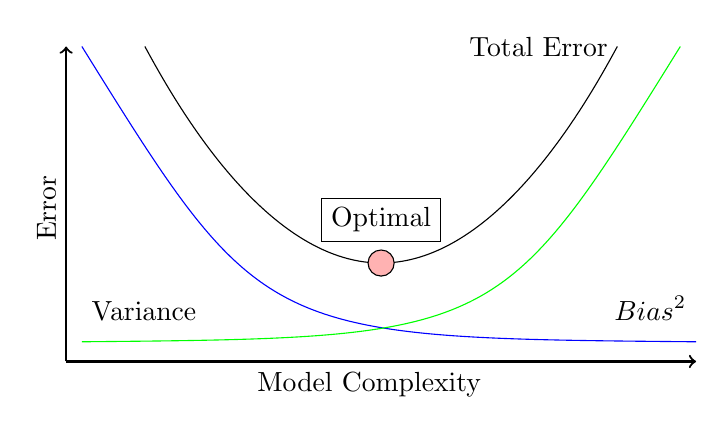
\begin{tikzpicture}[xscale=1,yscale=1]
            \draw[thick,->] (-4,0) -- (4,0) node[anchor=north east,xshift=-2.6cm]{Model Complexity};
            \draw[thick,->] (-4,0) -- (-4,4) node[anchor=south west,rotate=90,xshift=-2.6cm]{Error};
            % \draw[step=1cm,gray,very thin] (0,0) grid (4,4);
            % \draw[step=1cm,gray,very thin] (0,0) grid (-4,4);
            \draw[blue] (-3.8,4.00) .. controls (-1.5,0.3) .. (4.0,0.25);
            \node[anchor=south east,yshift=4pt] at (4,0.25){$\text{Bias}^2$};
            \draw[green] (-3.8,0.25) .. controls (+1.5,0.3) .. (3.8,4.00);
            \node[anchor=south west,yshift=4pt] at (-3.8,0.25){Variance};
            \draw (0,1.25) parabola (+3,4);
            \draw (0,1.25) parabola (-3,4);
            \node at (2,4){Total Error};
            \node[circle,draw,fill=red!30] at (0,1.25){};
            \node[draw] at (0,1.8){Optimal};
        \end{tikzpicture}
    \end{customcenter}
    Tuning parameters one can adjust bias and variance to find the optimal model.\\

    In classification we can use \textbf{the confusion matrix} to assess the performance of a model
    \begin{customcenter}[0pt]
        \begin{tabular}{ccc|c}
            & & \multicolumn{2}{c}{Predicted $\hat{y}$}\\
            & & {\scriptsize +} & - \\
            \multirow{2}{*}{\rotatebox[origin=c]{90}{Actual $y$}} & {\scriptsize +} & \cellcolor{gray!20} $\substack{\text{\textbf{TP}}\\\text{True Positives}}$ & \cellcolor{gray!40} $\substack{\text{\textcolor{gray!40}{Q}}\\ \text{\textbf{FN}}\\\text{False Negatives}\\\text{Type II Error}\\{}}$\\
            \cline{2-4}
            & - & \cellcolor{gray!40}
            $\substack{\text{\textcolor{gray!40}{Q}}\\\text{\textbf{FP}}\\\text{False Positives}\\\text{Type I Error}\\{}}$ & \cellcolor{gray!20} $\substack{\text{\textbf{TN}}\\\text{True Negatives}}$\\
        \end{tabular}
    \end{customcenter}
    \begin{customcenter}[5pt]
        \begin{tabular}{|l|c|l|}
            \hline
            \textbf{Metric} & \textbf{Formula} & \textbf{Interpretation} \\
            \hline
            \multirow{2}{*}{Accuracy} & \multirow{2}{*}{$\frac{\text{TP + TN}}{\text{T}^{\text{P}}_{\text{N}} + \text{F}^{\text{P}}_{\text{N}}}$} & \multirow{2}{*}{Overall performance of model} \\
            & & \\
            \hline
            \multirow{2}{*}{Precision} & \multirow{2}{*}{$\frac{\text{TP}}{\text{TP + FP}}$} & \multirow{2}{*}{Accuracy of \textbf{positive} predictions} \\
            & & \\
            \hline
            Recall & \multirow{2}{*}{$\frac{\text{TP}}{\text{TP + FN}}$} & \multirow{2}{*}{Coverage of actual \textbf{positive} sample} \\
            Sensitivity & & \\
            \hline
            \multirow{2}{*}{Specificity} & \multirow{2}{*}{$\frac{\text{TN}}{\text{TN + FN}}$} & \multirow{2}{*}{Coverage of actual \textbf{negative} sample} \\
            & & \\
            \hline
        \end{tabular}
    \end{customcenter}
    Some caveats about using machine learning as \textbf{silver bullet}
    \begin{itemize}
        \setlength\itemsep{0pt}
        \item Like humans, ML models make mistakes. Image recognition even being high accuracy (some around 95\%) the model will continue to give false positives.
        \item It is hard, if not impossible, to correct mistakes made by ML in a case-by-case manner. An error in ML is not like a bug in software development. % given that (1) ML does not \textit{manipulate} explicitly a model, and (2) modifying the model to fit a case commonly makes other cases to fail.
        \item It is hard, if not impossible, to reason about certain ML models. For example, \textbf{ResNet-50} consists of 50 layers of neurons with 25.6 million of parameters.
    \end{itemize}
\end{minipage}
%%%%%%%%%%%%%%%%%%%%%%%%%%%%%%%%%%%%